%%%%%%%%%%%%%%%%%%%%%%%%%%%%%%%%%%%%%%%%%%%
%%%%%%%%%%%%%%%%%%%%%%%%%%%%%%%%%%%%%%%%%%%
%%%%%%%%%%%%%%% CHAPTER 11 %%%%%%%%%%%%%%%%


\section{Erros estacionários em sistemas com realimentação unitária}

\frame{
\frametitle{Introdução}
\begin{block}{Contextualização}
A análise e o projeto de sistemas de controle estão focados em três especificações:
\begin{enumerate}
    \item Resposta transitória
    \item Estabilidade
    \item \textbf{Erros em regime permanente}
\end{enumerate}
\end{block}
}

\frame{
\frametitle{Introdução}
\begin{block}{Definição e entradas de teste}
O \textbf{erro em regime permanente (estacionário) é a diferença entre a entrada e a saída} para uma entrada prescrita quando $t \to \infty$. Lembrando que as entradas de testes que serão utilizadas são:
\begin{itemize}
    \item Degrau (posição constante)
    \item Rampa (velocidade constante)
    \item Parábola (aceleração constante)
\end{itemize}
\end{block}
}


\frame{
\frametitle{Introdução}
\centerline{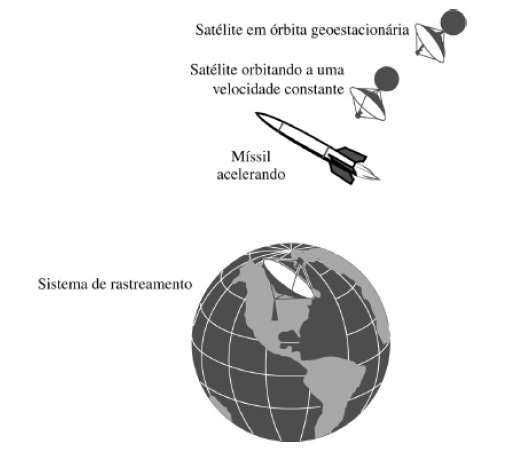
\includegraphics[width=0.7\linewidth]{Figuras/Ch11/fig1.PNG}}
}

\frame{
\frametitle{Introdução}
\begin{block}{Importante}
\begin{itemize}
    \item O erro estacionário é causado pela \textbf{incapacidade} de um sistema em seguir determinados tipos de \textbf{sinais de entradas}.
    \item Um sistema pode \textbf{não apresentar um erro estacionário a uma entrada em degrau}, mas o mesmo sistema \textbf{pode apresentar um erro estacionário não nulo a uma entrada em rampa}.
    \item A única maneira possível de eliminar esse erro é \textbf{modificando a estrutura do sistema}.
    \item O erro estacionário que um sistema apresenta em relação a determinado tipo de entrada depende do \textbf{tipo de função de transferência} desse sistema.
\end{itemize}
\end{block}
}

\frame{
\frametitle{Introdução}
\begin{block}{Aplicação a sistemas estáveis}
\begin{itemize}
    \item Nossa discussão é limitada aos \textbf{sistemas estáveis}, nos quais a resposta tende a zero à medida que $t \to \infty$.
    \item Os \textbf{sistemas instáveis} apresentam \textbf{perda de controle} em regime permanente e são absolutamente \textbf{inaceitáveis para utilização}.
    \item O erro é \textbf{medido verticalmente entre a entrada e a saída} após os transitórios terem desaparecido.
\end{itemize}
\end{block}
}

\frame{
\frametitle{Calculando erros em regime permanente}
\centerline{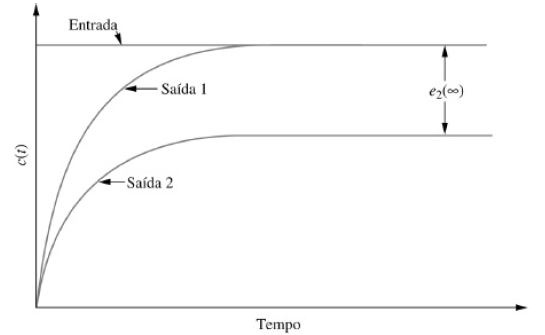
\includegraphics[width=0.7\linewidth]{Figuras/Ch11/fig2.PNG}}
\begin{block}{Ideia intuitiva para a entrada em degrau}
\begin{itemize}
    \item A saída 1 tem erro em regime permanente \textbf{nulo}.
    \item A saída 2 tem erro em regime permanente \textbf{finito}, $e_2(\infty)$.
\end{itemize}
\end{block}
}

\frame{
\frametitle{Calculando erros em regime permanente}
\centerline{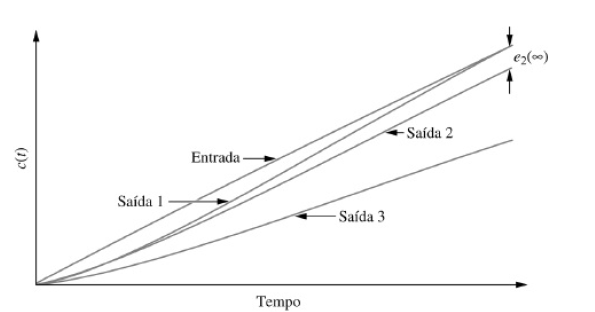
\includegraphics[width=0.7\linewidth]{Figuras/Ch11/fig3.PNG}}
\begin{block}{Ideia intuitiva para a entrada em rampa}
\begin{itemize}
    \item A saída 1 tem erro em regime permanente \textbf{nulo}.
    \item A saída 2 tem erro em regime permanente \textbf{finito}, $e_2(\infty)$.
    \item A saída 3 tem erro em regime permanente \textbf{infinito}, pois a inclinação da saída é diferente da inclinação da entrada.
\end{itemize}
\end{block}
}

\frame{
\frametitle{Erro em regime permanente para sistemas com realimentação unitária}
\begin{block}{Introdução}
O erro em regime permanente pode ser calculado a partir da função de transferência:
\begin{itemize}
    \item em \textbf{malha fechada} de um sistema, $T(s)$; ou
    \item em \textbf{malha aberta}, $G(s)$, para sistemas com realimentação unitária.
\end{itemize}
\end{block}
}

\frame{
\frametitle{Erro em regime permanente para sistemas com realimentação unitária}
\centerline{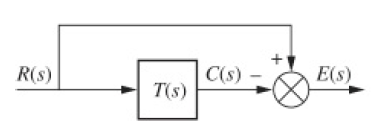
\includegraphics[width=0.5\linewidth]{Figuras/Ch11/fig4.PNG}}
\begin{block}{Erro em regime permanente em função de $T(s)$}
$$E(s) = R(s) - C(s)$$
Mas
$$C(s) = R(s) \cdot T(s)$$
Deste modo,
$$\boxed{E(s) = R(s)\Big(1 - T(s)\Big)}$$
\end{block}
}

\frame{
\frametitle{Erro em regime permanente para sistemas com realimentação unitária}
\begin{block}{Erro em regime permanente em função de $T(s)$}
\begin{itemize}
    \item Estamos interessados no \textbf{valor final do erro}, $e(\infty)$.
\end{itemize}
Aplicando o teorema do valor final\footnote{Válido somente se $E(s)$ possui polos apenas no semiplano da esquerda e na origem, e a função de transferência em malha fechada, $T(s)$, for estável.}, obtemos:
$$e(\infty) = \lim_{t\to\infty} e(t) = \lim_{s\to 0} sE(s)$$
Substituindo a equação anterior nesta, temos:
$$\boxed{e(\infty) = \lim_{s\to 0} s R(s)\Big(1 - T(s)\Big)}$$
\end{block}
}

\frame{
\frametitle{Exemplo $\#01$ - erro em regime permanente em função de $T(s)$}
\begin{block}{}
Determine o erro em regime permanente considerando que a entrada seja um degrau unitário e que 
$$T(s) = \dfrac{5}{s^2+7s+10}$$
\vspace{0.5cm}
\textbf{Resolução:}
$$e(\infty) = \lim_{s\to 0} s R(s)\Big(1 - T(s)\Big) = \lim_{s\to 0} s \dfrac{1}{s}\Big(1 - \dfrac{5}{s^2+7s+10}\Big)$$
Manipulando a equação acima, obtemos:
$$e(\infty) = \lim_{s\to 0} \dfrac{s^2+7s+5}{s^2+7s+10} = \dfrac{1}{2}$$
\end{block}
}

\frame{
\frametitle{Erro em regime permanente para sistemas com realimentação unitária}
\centerline{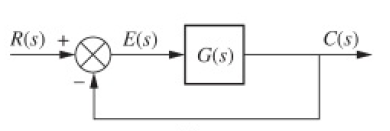
\includegraphics[width=0.5\linewidth]{Figuras/Ch11/fig5.PNG}}
\begin{block}{Erro em regime permanente em função de $G(s)$}
$$E(s) = R(s) - C(s)$$
Mas
$$C(s) = E(s) \cdot G(s)$$
Deste modo,
$$E(s) = R(s) - E(s) \cdot G(s)$$
$$\boxed{E(s) = \dfrac{R(s)}{1+G(s)}}$$
\end{block}
}

\frame{
\frametitle{Erro em regime permanente para sistemas com realimentação unitária}
\begin{block}{Erro em regime permanente em função de $G(s)$}
\begin{itemize}
    \item Estamos interessados no \textbf{valor final do erro}, $e(\infty)$.
\end{itemize}
Aplicando o teorema do valor final\footnote{Neste ponto em um cálculo numérico, devemos verificar se o sistema em malha fechada é estável.}, obtemos:
$$e(\infty) = \lim_{t\to\infty} e(t) = \lim_{s\to 0} sE(s)$$
Substituindo a equação anterior nesta, temos:
$$\boxed{e(\infty) = \lim_{s\to 0} \dfrac{sR(s)}{1+G(s)}}$$
\vspace{-0.4cm}
\begin{itemize}
    \item Esta equação nos permite calcular $e(\infty)$ dados a entrada e o sistema. Vamos analisar agora diversas \textbf{entradas} $R(s)$ e observar as relações que existem entre o sistema em malha aberta e a \textbf{natureza do erro}.
\end{itemize}
\end{block}
}

\frame{
\frametitle{Erro em regime permanente para sistemas com realimentação unitária}
\begin{block}{Erro em regime permanente em função de $G(s)$ - entrada em \textbf{degrau}}
$$e(\infty) = \lim_{s\to 0} \dfrac{sR(s)}{1+G(s)}$$
Como estamos analisando o erro para uma \textbf{entrada em degrau}, temos:
$$R(s) = \dfrac{1}{s}$$
Deste modo,
$$\boxed{e(\infty) = \lim_{s\to 0} \dfrac{s(1/s)}{1+G(s)} = \dfrac{1}{1 + \lim_{s\to 0} G(s)}}$$
\end{block}
}

\frame{
\frametitle{Erro em regime permanente para sistemas com realimentação unitária}
\begin{block}{Erro em regime permanente em função de $G(s)$ - entrada em \textbf{degrau}}
\begin{itemize}
    \item Para termos \textbf{erro em regime permanente nulo},
\end{itemize}
$$\lim_{s\to 0} G(s) = \infty$$
Portanto, para satisfazer a equação anterior, $G(s)$ deve ter a seguinte forma:
$$G(s) = \dfrac{(s+z_1)(s+z_2)\cdots}{s^n(s+p_1)(s+p_2)\cdots}, n \geq 1$$
Em outras palavras, \textbf{pelo menos um polo deve estar na origem}. Lembrando que a divisão por $s$ no domínio da frequência corresponde à integração no domínio do tempo, podemos falar que o erro em regime permanente será nulo caso haja \textbf{pelo menos uma integração}.
\end{block}
}

\frame{
\frametitle{Erro em regime permanente para sistemas com realimentação unitária}
\begin{block}{Erro em regime permanente em função de $G(s)$ - entrada em \textbf{degrau}}
\begin{itemize}
    \item Para termos \textbf{erro em regime permanente constante},
\end{itemize}
$$\lim_{s\to 0} G(s) = K, \ \text{onde $K$ é uma constante}$$
Portanto, para satisfazer a equação anterior, $G(s)$ deve ter a seguinte forma:
$$G(s) = \dfrac{(s+z_1)(s+z_2)\cdots}{(s+p_1)(s+p_2)\cdots}$$
Em outras palavras, \textbf{não há a presença de polos na origem}. Lembrando que a divisão por $s$ no domínio da frequência corresponde à integração no domínio do tempo, podemos falar que o erro em regime permanente será constante caso \textbf{não haja integrações}.
\end{block}
}

\frame{
\frametitle{Erro em regime permanente para sistemas com realimentação unitária}
\begin{block}{Erro em regime permanente em função de $G(s)$ - entrada em \textbf{rampa}}
$$e(\infty) = \lim_{s\to 0} \dfrac{sR(s)}{1+G(s)}$$
Como estamos analisando o erro para uma \textbf{entrada em rampa}, temos:
$$R(s) = \dfrac{1}{s^2}$$
Deste modo,
$$\boxed{e(\infty) = \lim_{s\to 0} \dfrac{s(1/s^2)}{1+G(s)} = \lim_{s\to 0} \dfrac{1}{s+sG(s)} = \dfrac{1}{\lim_{s\to 0} sG(s)}}$$
\end{block}
}

\frame{
\frametitle{Erro em regime permanente para sistemas com realimentação unitária}
\begin{block}{Erro em regime permanente em função de $G(s)$ - entrada em \textbf{rampa}}
\begin{itemize}
    \item Para termos \textbf{erro em regime permanente nulo},
\end{itemize}
$$\lim_{s\to 0} sG(s) = \infty$$
Portanto, para satisfazer a equação anterior, $G(s)$ deve ter a seguinte forma:
$$G(s) = \dfrac{(s+z_1)(s+z_2)\cdots}{s^n(s+p_1)(s+p_2)\cdots}, n \geq 2$$
Em outras palavras, \textbf{pelo menos dois polos devem estar na origem}. Lembrando que a divisão por $s$ no domínio da frequência corresponde à integração no domínio do tempo, podemos falar que o erro em regime permanente será nulo caso haja \textbf{pelo menos duas integrações}.
\end{block}
}

\frame{
\frametitle{Erro em regime permanente para sistemas com realimentação unitária}
\begin{block}{Erro em regime permanente em função de $G(s)$ - entrada em \textbf{rampa}}
\begin{itemize}
    \item Para termos \textbf{erro em regime permanente constante},
\end{itemize}
$$\lim_{s\to 0} sG(s) = K, \ \text{onde $K$ é uma constante}$$
Portanto, para satisfazer a equação anterior, $G(s)$ deve ter a seguinte forma:
$$G(s) = \dfrac{(s+z_1)(s+z_2)\cdots}{s(s+p_1)(s+p_2)\cdots}$$
Em outras palavras, \textbf{há a presença de um polo na origem}. Lembrando que a divisão por $s$ no domínio da frequência corresponde à integração no domínio do tempo, podemos falar que o erro em regime permanente será constante caso \textbf{haja apenas uma integração}.
\end{block}
}

\frame{
\frametitle{Erro em regime permanente para sistemas com realimentação unitária}
\begin{block}{Erro em regime permanente em função de $G(s)$ - entrada em \textbf{rampa}}
\begin{itemize}
    \item Para termos \textbf{erro em regime permanente infinito},
\end{itemize}
$$\lim_{s\to 0} sG(s) = 0$$
Portanto, para satisfazer a equação anterior, $G(s)$ deve ter a seguinte forma:
$$G(s) = \dfrac{(s+z_1)(s+z_2)\cdots}{(s+p_1)(s+p_2)\cdots}$$
Em outras palavras, \textbf{não há a presença de polos na origem}. Lembrando que a divisão por $s$ no domínio da frequência corresponde à integração no domínio do tempo, podemos falar que o erro em regime permanente será infinito caso \textbf{não haja integrações}.
\end{block}
}

\frame{
\frametitle{Erro em regime permanente para sistemas com realimentação unitária}
\begin{block}{Erro em regime permanente em função de $G(s)$ - entrada em \textbf{parábola}}
$$e(\infty) = \lim_{s\to 0} \dfrac{sR(s)}{1+G(s)}$$
Como estamos analisando o erro para uma \textbf{entrada em parábola}, temos:
$$R(s) = \dfrac{1}{s^3}$$
Deste modo,
$$\boxed{e(\infty) = \lim_{s\to 0} \dfrac{s(1/s^3)}{1+G(s)} = \lim_{s\to 0} \dfrac{1}{s^2+s^2G(s)} = \dfrac{1}{\lim_{s\to 0} s^2G(s)}}$$
\end{block}
}

\frame{
\frametitle{Erro em regime permanente para sistemas com realimentação unitária}
\begin{block}{Erro em regime permanente em função de $G(s)$ - entrada em \textbf{parábola}}
\begin{itemize}
    \item Para termos \textbf{erro em regime permanente nulo},
\end{itemize}
$$\lim_{s\to 0} s^2G(s) = \infty$$
Portanto, para satisfazer a equação anterior, $G(s)$ deve ter a seguinte forma:
$$G(s) = \dfrac{(s+z_1)(s+z_2)\cdots}{s^n(s+p_1)(s+p_2)\cdots}, n \geq 3$$
Em outras palavras, \textbf{pelo menos três polos devem estar na origem}. Lembrando que a divisão por $s$ no domínio da frequência corresponde à integração no domínio do tempo, podemos falar que o erro em regime permanente será nulo caso haja \textbf{pelo menos três integrações}.
\end{block}
}

\frame{
\frametitle{Erro em regime permanente para sistemas com realimentação unitária}
\begin{block}{Erro em regime permanente em função de $G(s)$ - entrada em \textbf{parábola}}
\begin{itemize}
    \item Para termos \textbf{erro em regime permanente constante},
\end{itemize}
$$\lim_{s\to 0} s^2G(s) = K, \ \text{onde $K$ é uma constante}$$
Portanto, para satisfazer a equação anterior, $G(s)$ deve ter a seguinte forma:
$$G(s) = \dfrac{(s+z_1)(s+z_2)\cdots}{s^2(s+p_1)(s+p_2)\cdots}$$
Em outras palavras, \textbf{há a presença de dois polos na origem}. Lembrando que a divisão por $s$ no domínio da frequência corresponde à integração no domínio do tempo, podemos falar que o erro em regime permanente será constante caso \textbf{haja duas integrações}.
\end{block}
}

\frame{
\frametitle{Erro em regime permanente para sistemas com realimentação unitária}
\begin{block}{Erro em regime permanente em função de $G(s)$ - entrada em \textbf{parábola}}
\begin{itemize}
    \item Para termos \textbf{erro em regime permanente infinito},
\end{itemize}
$$\lim_{s\to 0} s^2G(s) = 0$$
Portanto, para satisfazer a equação anterior, $G(s)$ deve ter a seguinte forma:
$$G(s) = \dfrac{(s+z_1)(s+z_2)\cdots}{s(s+p_1)(s+p_2)\cdots}$$
Em outras palavras, \textbf{há a presença de um ou nenhum polo na origem}. Lembrando que a divisão por $s$ no domínio da frequência corresponde à integração no domínio do tempo, podemos falar que o erro em regime permanente será infinito caso \textbf{haja uma ou nenhuma integração}.
\end{block}
}

\frame{
\frametitle{Exemplo $\#02$ - erro em regime permanente em função de $G(s)$}
\begin{block}{}
Determine os erros em regime permanente para entradas de $5u(t)$, $5tu(t)$ e $5t^2u(t)$, considerando que a função $u(t)$ é o degrau unitário e que 
$$G(s) = \dfrac{120(s+2)}{(s+3)(s+4)}$$
\vspace{-0.1cm}
\textbf{Resolução:}
\begin{itemize}
    \item Para a entrada em degrau (de \textbf{amplitude} 5):
\end{itemize}
$$e(\infty) = \dfrac{5}{1 + \lim_{s\to 0} G(s)} = \dfrac{5}{1 + 20} = \dfrac{5}{21}$$
\vspace{-0.2cm}
\begin{itemize}
    \item Para a entrada em rampa (de \textbf{amplitude} 5):
\end{itemize}
$$e(\infty) = \dfrac{5}{\lim_{s\to 0} sG(s)} = \dfrac{5}{0} = \infty$$
\vspace{-0.2cm}
\begin{itemize}
    \item Para a entrada em parábola (de \textbf{amplitude} 10):
\end{itemize}
$$e(\infty) = \dfrac{10}{\lim_{s\to 0} s^2G(s)} = \dfrac{10}{0} = \infty$$
\end{block}
}

\frame{
\frametitle{Exemplo $\#03$ - erro em regime permanente em função de $G(s)$}
\begin{block}{}
Determine os erros em regime permanente para entradas de $5u(t)$, $5tu(t)$ e $5t^2u(t)$, considerando que a função $u(t)$ é o degrau unitário e que 
$$G(s) = \dfrac{100(s+2)(s+6)}{s(s+3)(s+4)}$$
\vspace{-0.1cm}
\textbf{Resolução:}
\begin{itemize}
    \item Para a entrada em degrau (de \textbf{amplitude} 5):
\end{itemize}
$$e(\infty) = \dfrac{5}{1 + \lim_{s\to 0} G(s)} = \dfrac{5}{1 + \infty} = 0$$
\vspace{-0.2cm}
\begin{itemize}
    \item Para a entrada em rampa (de \textbf{amplitude} 5):
\end{itemize}
$$e(\infty) = \dfrac{5}{\lim_{s\to 0} sG(s)} = \dfrac{5}{100} = \dfrac{1}{20}$$
\vspace{-0.2cm}
\begin{itemize}
    \item Para a entrada em parábola (de \textbf{amplitude} 10):
\end{itemize}
$$e(\infty) = \dfrac{10}{\lim_{s\to 0} s^2G(s)} = \dfrac{10}{0} = \infty$$
\end{block}
}

\frame{
\frametitle{Constantes de erro estático e tipo do sistema}
\begin{block}{Introdução}
\begin{itemize}
    \item Quando tratamos das \textbf{especificações de desempenho} para a \textbf{resposta transitória} definimos fator de amortecimento, frequência natural, tempo de acomodação, \textit{overshoot}, etc.
    \item E para o \textbf{regime permanente}? Essas especificações de desempenho de erro em regime permanente são chamadas de \textbf{constantes de erro estático}.
\end{itemize}
\end{block}
}

\frame{
\frametitle{Constantes de erro estático e tipo do sistema}
\begin{block}{Constantes de erro estático}
\begin{itemize}
    \item O erro em regime permanente para uma \textbf{entrada em degrau} foi deduzido como
\end{itemize}
$$e(\infty) = \dfrac{1}{1 + \lim_{s\to 0} G(s)}$$
O termo no \textbf{denominador}, para o qual se calcula o limite, determina o \textbf{erro em regime permanente}. Chamamos esse limite de \textbf{constante de erro estático de posição}, $K_p$:
$$\boxed{K_p = \lim_{s\to 0} G(s)}$$
Deste modo,
$$e(\infty) = \dfrac{1}{1 + K_p}$$
\end{block}
}

\frame{
\frametitle{Constantes de erro estático e tipo do sistema}
\begin{block}{Constantes de erro estático}
\begin{itemize}
    \item O erro em regime permanente para uma \textbf{entrada em rampa} foi deduzido como
\end{itemize}
$$e(\infty) = \dfrac{1}{\lim_{s\to 0} sG(s)}$$
O termo no \textbf{denominador}, para o qual se calcula o limite, determina o \textbf{erro em regime permanente}. Chamamos esse limite de \textbf{constante de erro estático de velocidade}, $K_v$:
$$\boxed{K_v = \lim_{s\to 0} sG(s)}$$
Deste modo,
$$e(\infty) = \dfrac{1}{K_v}$$
\end{block}
}

\frame{
\frametitle{Constantes de erro estático e tipo do sistema}
\begin{block}{Constantes de erro estático}
\begin{itemize}
    \item O erro em regime permanente para uma \textbf{entrada em parábola} foi deduzido como
\end{itemize}
$$e(\infty) = \dfrac{1}{\lim_{s\to 0} s^2G(s)}$$
O termo no \textbf{denominador}, para o qual se calcula o limite, determina o \textbf{erro em regime permanente}. Chamamos esse limite de \textbf{constante de erro estático de aceleração}, $K_a$:
$$\boxed{K_a = \lim_{s\to 0} s^2G(s)}$$
Deste modo,
$$e(\infty) = \dfrac{1}{K_a}$$
\end{block}
}

\frame{
\frametitle{Exemplo $\#04$ - erro em regime permanente em função de $G(s)$}
\begin{block}{}
Determine as constantes de erro estático e obtenha o erro esperado para as entradas padronizadas em degrau, em rampa, e em parábola, considerando que 
$$G(s) = \dfrac{500(s+2)(s+4)(s+5)(s+6)(s+7)}{s^2(s+8)(s+10)(s+12)}$$
\vspace{-0.1cm}
\textbf{Resolução:}
\begin{itemize}
    \item Para a entrada em degrau:
\end{itemize}
$$K_p = \lim_{s\to 0} G(s) = \infty \implies e(\infty) = \dfrac{1}{1 + K_p} = \dfrac{1}{1 + \infty} = 0$$
\vspace{-0.2cm}
\begin{itemize}
    \item Para a entrada em rampa:
\end{itemize}
$$K_v = \lim_{s\to 0} sG(s) = \infty \implies e(\infty) = \dfrac{1}{K_v} = \dfrac{1}{\infty} = 0$$
\vspace{-0.2cm}
\begin{itemize}
    \item Para a entrada em parábola:
\end{itemize}
$$K_a = \lim_{s\to 0} s^2G(s) = 875 \implies e(\infty) = \dfrac{1}{K_a} = \dfrac{1}{875} = 0,00114$$
\end{block}
}

\frame{
\frametitle{Constantes de erro estático e tipo do sistema}
\begin{block}{Tipo do sistema}
\begin{itemize}
    \item Os valores das constantes de erro estático, novamente, dependem da forma de $G(s)$, especialmente do \textbf{número de integrações} existentes no ramo direto.
\end{itemize}
Dado
$$G(s) = \dfrac{K(s+z_1)(s+z_2)+\cdots}{s^n(s+p_1)(s+p_2)+\cdots}$$
definimos o \textbf{tipo de sistema} como valor de $n$ no denominador ou, equivalentemente, o \textbf{número de integrações} existentes no ramo direto.
\end{block}
}

\frame{
\frametitle{Constantes de erro estático e tipo do sistema}
\centerline{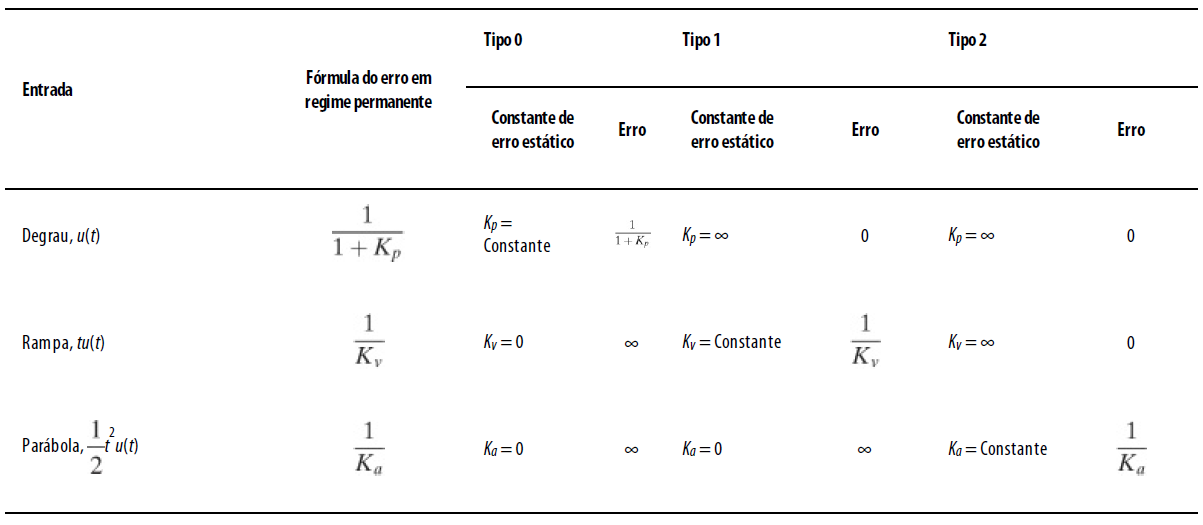
\includegraphics[width=1.2\linewidth]{Figuras/Ch11/fig6.PNG}}
}

\frame{
\frametitle{Exemplo $\#05$ - projeto de ganho para atender a uma especificação de desempenho de erro em regime permanente}
\begin{block}{}
Dado
$$G(s) = \dfrac{K(s+5)}{s(s+6)(s+7)(s+8)}$$
determine o valor de $K$ de modo que haja um erro de $10\%$ em regime permanente. \\
\vspace{0.2cm}
\textbf{Resolução:} \\
\vspace{0.2cm}
Como o sistema é do Tipo 1, o erro declarado no problema deve se aplicar a uma entrada em rampa.
$$e(\infty) = \dfrac{1}{K_v} = 0,1 \implies K_v = 10$$
Portanto,
$$K_v = \lim_{s\to 0} sG(s) = \dfrac{K \cdot 5}{6 \cdot 7 \cdot 8} = \dfrac{5K}{336} = 10 \ \therefore \ K = 672$$
\end{block}
}

\frame{
\frametitle{Exercícios}
\begin{block}{}
01. Avalie a resposta de regime permanente do sistema de realimentação unitária cuja função de transferência $G(s)$ é:
$$G(s) = \dfrac{s+12}{s(s+1)(s+3)}$$

\vspace{0.1cm}

02. Determine o valor de $K$ para resultar em um erro de $10\%$ em regime permanente para um sistema que possui a seguinte função de transferência:
$$G(s) = \dfrac{K(s+12)}{(s+14)(s+18)}$$

\vspace{0.1cm}

03. Determine o tipo do sistema para o sistema da figura abaixo.
\end{block}
\centerline{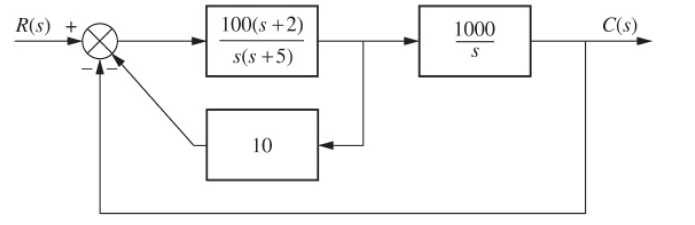
\includegraphics[width=0.57\linewidth]{Figuras/Ch11/fig7.PNG}}
}

\frame{
\frametitle{Referências e exercícios complementares}
\begin{itemize}
\item NISE, Norman S. Engenharia de Sistemas de Controle, 7 ed. LTC, 2017.
\end{itemize}
\centering{\alert{Página 304 - \textbf{Capítulo 7}}} \\
\vspace{0.4cm}
\begin{itemize}
\item OGATA, Katsuhiko. Engenharia de Controle Moderno, 5 ed. Pearson, 2010.
\end{itemize}
\centering{\alert{Página 238 - \textbf{Capítulo 5}}} \\
}